\chapter{Elementos da F\'isica-Matem\'atica}

\section{EDP de uma Onda}
Segundo \cite{farlow_93}, a EDP de uma onda 
\begin{equation}\label{eq.edp_geral}
\frac{\partial^2\mathbf{f}(\mathbf{x},t)}{\partial\,t^2}=\norm{\mathbf{v}}^2\nabla^2\mathbf{f}(\mathbf{x},t)
\end{equation}
possui a solu\c{c}\~ao de D'Alembert
\begin{equation}
\mathbf{f}(\mathbf{x},t)=\mathbf{g}_1(\mathbf{x}-\mathbf{v}\,t)+\mathbf{g}_2(\mathbf{x}+\mathbf{v}\,t),
\end{equation}
onde $\mathbf{x}=(x,y,z)^\top$ representa o espa\c{c}o $\mathbb{R}^3$, $\mathbf{v}$ \'e a \textit{velocidade} de propaga\c{c}\~ao da onda, $(\mathbf{x}\pm\mathbf{v}\,t)$ \'e a \textit{fase} da onda, $\mathbf{g}_1$ \'e a propaga\c{c}\~ao da onda no semiespa\c{c}o positivo do eixo $x$ e $\mathbf{g}_2$ \'e a propaga\c{c}\~ao da onda no semiespa\c{c}o negativo do eixo $x$.

De acordo com \cite{chew}, ondas tridimensionais oriundas de fonte pontual se propagam em formato esferoidal mas localmente podem ser tratadas como ondas planas, principalmente para raios distantes da fonte. A onda esf\'erica, solu\c{c}\~ao da EDP \ref{eq.edp_geral}, pode ser representada pela superposi\c{c}\~ao de ondas planas atrav\'es da identidade de \textit{Weyl}, onde tal superposi\c{c}\~ao tamb\'em \'e solu\c{c}\~ao da EDP \ref{eq.edp_geral}, conforme \cite{weyl_19}.

No $\mathbb{R}^3$ o \textit{vetor de onda} $\mathbf{k}=(k_x,k_y,k_z)^\top$ \'e aquele que aponta na dire\c{c}\~ao de propaga\c{c}\~ao da onda e sua magnitude, denominada \textit{n\'umero de onda}, \'e definida como 
\begin{equation}
\norm{\mathbf{k}}=k=\frac{\omega}{\norm{\mathbf{v}}},
\end{equation}
onde $\omega$ \'e a frequ\^encia temporal. Desta forma, a fase da onda pode ser escrita em termos do vetor de onda e da frequ\^encia como $(\mathbf{k}\cdot\mathbf{x}-\omega\,t)$, e a solu\c{c}\~ao da equa\c{c}\~ao \ref{eq.edp_geral} pode ser reescrita como uma superposi\c{c}\~ao de ondas planas
\begin{equation}
\mathbf{f}(\mathbf{x},t)=\mathbf{A}\,\sum_{\mathbf{k},\omega}{e^{i\,(\mathbf{k}\cdot\mathbf{x}-\omega\,t)}},
\end{equation}
onde $\mathbf{A}$ \'e a \textit{amplitude} da onda.

Podemos verificar em \cite{White_Zhou_2006}, para o caso $\mathbb{R}^2$ o \textit{vetor de onda horizontal} \'e definido como $\mathbf{k}=(k_x,k_y)^\top$, o \textit{n\'umero de onda horizontal} e a \textit{vagarosidade horizontal} s\~ao, respectivamente,
\begin{equation}\label{eq.numero_onda_vagarozidade_horizontal}
k=\sqrt{k_x^2+k_y^2}\qquad\text{e}\qquad\gamma=\frac{k}{\omega}.
\end{equation}
A vagarosidade vertical \'e definida como
\begin{equation}
q_0=\frac{1}{v_z},
\end{equation}
onde $v_z$ \'e a componente vertical da velocidade. Denotando o \textit{n\'umero de onda vertical} por $k_z$, temos que a \textit{vagarosidade vertical} pode ser escrita como
\begin{equation}
q_0=\frac{k_z}{\omega}.
\end{equation}
Combinando as vagarosidades horizontal e vertical, temos
\begin{equation}\label{eq.vagarosidade_vertical}
\gamma^2+q_0^2=\frac{1}{\norm{\mathbf{v}}^2}\qquad\text{ou}\qquad q_0=\sqrt{\epsilon_0\mu_0-\gamma^2},
\end{equation}
j\'a que $\epsilon_0\mu_0=\frac{1}{\norm{\mathbf{v}}^2}$.

\section{Transformadas Laterais de Fourier}

Segundo \cite{butkov_88}, podemos definir as transformadas laterais de Fourier direta e inversa entre o espa\c{c}o bidimensional e o vetor de onda horizontal como
\begin{align}\label{eq.trans_fourier_1}
\mathbf{\widehat{f}}(k_x,k_y,z) &= \iint_{\mathbb{R}^2}\mathbf{f}(x,y,z)\,e^{-i(k_xx+k_yy)}dx\,dy\\\nonumber\\\label{eq.trans_fourier_2}
\mathbf{f}(x,y,z) &= \left(\frac{1}{2\,\pi}\right)^2\iint_{\mathbb{R}^2}\mathbf{\widehat{f}}(k_x,k_y,z)\,e^{i(k_xx+k_yy)}dk_xdk_y.
\end{align}
O s\'imbolo $\,\widehat{}\,$ denota a fun\c{c}\~ao no espa\c{c}o da transformada lateral de Fourier.

A propriedade da transformada de derivadas \'e a que mais nos interessa e, supondo $f$ uma fun\c{c}\~ao escalar de uma \'unica vari\'avel, essa propriedade pode ser descrita como  
\begin{align*}
\widehat{f'}(x)&=\int_{-\infty}^{\infty}f'(x)\,e^{-i\,k_xx}dx\\
&=f(x)\,e^{-i\,k_xx}|_{-\infty}^{\infty}-(-i\,k_x)\int_{-\infty}^{\infty}f(x)\,e^{-i\,k_xx}dx\\
&=i\,k_x\widehat{f}(k_x).
\end{align*}
Na passagem da segunda para a terceira igualdade utilizamos a hip\'otese bastante difundida em geof\'isica de que $f(x)\rightarrow 0$ quando $x \rightarrow \pm \infty $, a qual podemos observar em demonstra\c{c}\~oes de teoremas como, por exemplo, o toerema de \textit{Helmholtz} encontrado em \cite{griffiths}. 


\section{Rota\c{c}\~oes}

Segundo \cite{lang_1986}, podemos produzir uma rota\c{c}\~ao antihor\'aria em torno do eixo $z$ aplicando o operador linear
\begin{equation*}
\begin{pmatrix}
\cos\theta&-\sin\theta&0\\
\sin\theta&\cos\theta&0\\
0&0&1
\end{pmatrix},
\end{equation*}
onde $\theta$ \'e o \^angulo que um vetor est\'a sendo rotacionado. Como a geometria do nosso problema considera ondas se propagando na parte negativa do eixo $z$ (consideramos $z$ positivo no sentido descendente), para produzirmos uma rota\c{c}\~ao antihor\'aria devemos considerar o \^angulo $-\theta$, e com isso nossa matriz de rota\c{c}\~ao se torna
\begin{equation*}
\begin{pmatrix}
\cos\theta&\sin\theta&0\\
-\sin\theta&\cos\theta&0\\
0&0&1
\end{pmatrix},
\end{equation*}
lembrando a paridade das fun\c{c}\~oes seno e cosseno. Para promovermos uma rota\c{c}\~ao orientando a primeira coordenada  no sentido de propaga\c{c}\~ao das ondas horizontais, temos que $\theta$ ser\'a o \^angulo entre $(x,0,0)^\top$ e $(k_x,k_y,0)^\top$, e a matriz de rota\c{c}\~ao se torna
\begin{equation}\label{eq.operador_rotacao}
\Omega=
\begin{pmatrix}
\frac{k_x}{k}&\frac{k_y}{k}&0\\
-\frac{k_y}{k}&\frac{k_x}{k}&0\\
0&0&1
\end{pmatrix}.
\end{equation}
Para escrevermos novamente as equa\c{c}\~oes no sistema de coordenadas original, precisamos aplicar a rota\c{c}\~ao inversa. Para isso, basta inverter a matriz de rota\c{c}\~ao \ref{eq.operador_rotacao} mas, como se trata de uma matriz ortogonal, a inversa \'e a sua transposta. Assim, usaremos
\begin{equation}\label{eq.rotacao_inversa}
\Omega^\top=
\begin{pmatrix}
\frac{k_x}{k}&-\frac{k_y}{k}&0\\
\frac{k_y}{k}&\frac{k_x}{k}&0\\
0&0&1
\end{pmatrix}.
\end{equation}


A rota\c{c}\~ao de um tensor $\tau$ \'e dada por 
\begin{equation}\label{eq.rotacao_tensor}
\tilde{\tau}=\Omega\,\tau\,\Omega^\top,
\end{equation}
e sua rota\c{c}\~ao inversa \'e dada por
\begin{equation}\label{eq.rot_inver_tensor}
\tau=\Omega^\top\tilde{\tau}\,\Omega.
\end{equation}


\section{A fun\c{c}\~ao $\delta$ de Dirac}\label{sec.dirac}

Em algumas aplica\c{c}\~oes f\'isicas pode ser necess\'ario trabalhar com conceito de um pulso de dura\c{c}\~ao infinitamente curta. De acordo com \cite{butkov_88}, podemos tomar o exemplo de um corpo colocado em movimento, a partir do repouso, atrav\'es de um golpe instant\^aneo que faz o mesmo adquirir um momento igual \`a impuls\~ao $I$ do choque, ou seja,
\begin{equation}
I=\int_{t_0}^{t_0+\Delta\,t}f(t)dt,
\end{equation}
onde $f(t)$ \'e a for\c{c}a e $\Delta\,t$ \'e o tempo de a\c{c}\~ao da for\c{c}a. A implus\~ao \'e um n\'umero finito e sua altera\c{c}\~ao ocorre instantaneamente, pois $\Delta\,t$ \'e um n\'umero muito pequeno. Assim, temos que a for\c{c}a deveria ter valor infinito durante o golpe e nula nos outros instantes, conforme o gr\'afico da figura \ref{fig.dirac}.
\begin{figure}
\centering
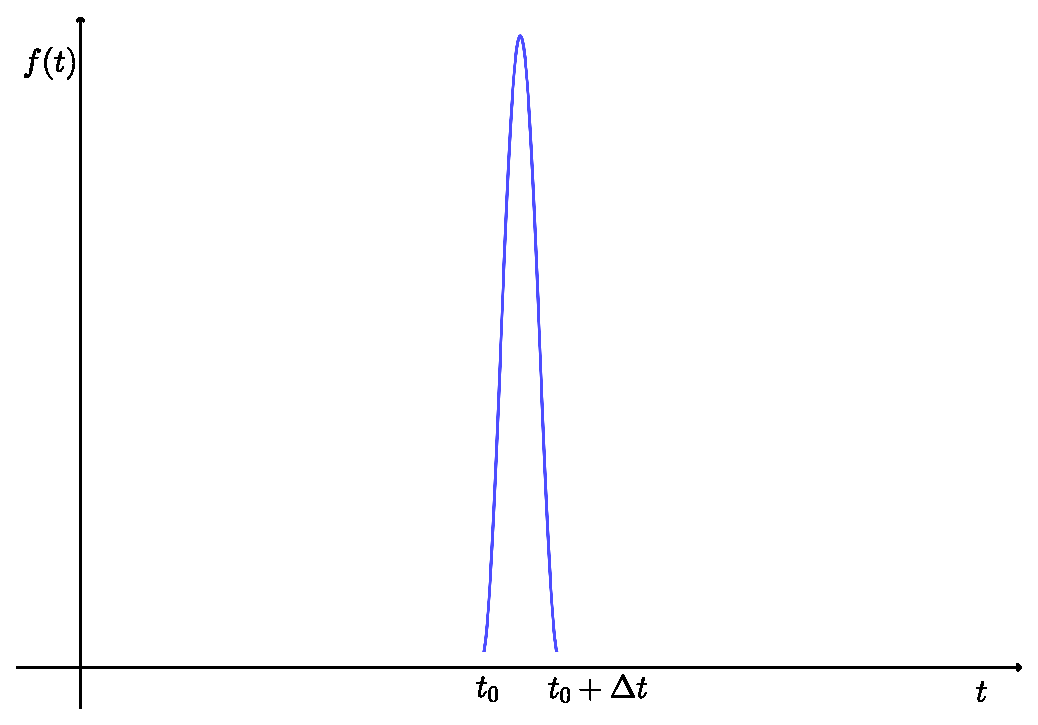
\includegraphics[scale=.6]{dirac_function}
\caption{\textit{Representa\c{c}\~ao de uma fun\c{c}\~ao fortemente concentrada.}}
\label{fig.dirac}
\end{figure}
A fim de facilitar v\'arias opera\c{c}\~oes da f\'isica-matem\'atica, Dirac prop\^os a introdu\c{c}\~ao da chamada fun\c{c}\~ao $\delta(x)$, que pode representar uma fun\c{c}\~ao infinitamente concentrada e \'e dada simbolicamente por
\begin{empheq}[left={\delta(x)=\empheqlbrace}]{align*}
0\,,&\quad\text{se}\quad x\neq 0\\
\infty\,,&\quad\text{se}\quad x=0
\end{empheq}
e $\delta$ deve satisfazer a seguinte condi\c{c}\~ao
\begin{equation}\label{eq.condicao_dirac}
\int_{-\infty}^{\infty}\delta(x)\,dx=1.
\end{equation}
Sendo $f$ uma fun\c{c}\~ao cont\'inua qualquer, a utilidade da fun\c{c}\~ao $\delta$ consiste em determinar o valor de 
\begin{equation}
\int_{-\infty}^{\infty}\delta(x)\,f(x)\,dx
\end{equation}
substituindo os limites de integra\c{c}\~ao por $-\epsilon$ e $\epsilon$, onde $\epsilon$ \'e um n\'umero positivo infinitesimalmente pr\'oximo de zero. Tal substitui\c{c}\~ao se justifica pois $\delta=0$ se $x\neq0$ e teremos uma aproxima\c{c}\~ao para o valor dessa integral. Assim, usando a defini\c{c}\~ao de $\delta$, a condi\c{c}\~ao \ref{eq.condicao_dirac} e a continuidade de $f$, temos
\begin{align*}
\int_{-\infty}^{\infty}\delta(x)\,f(x)\,dx&=\int_{-\infty}^{-\epsilon}\delta(x)\,f(x)\,dx+\int_{-\epsilon}^{\epsilon}\delta(x)\,f(x)\,dx+\int_{\epsilon}^{\infty}\delta(x)\,f(x)\,dx\\
&=\int_{-\epsilon}^{\epsilon}\delta(x)\,f(x)\,dx\\
&\approx\,f(0)\int_{-\epsilon}^{\epsilon}\delta(x)\,dx\\
&=f(0).
\end{align*}
Desta forma podemos representar a aplica\c{c}\~ao de uma fun\c{c}\~ao fortemente concentrada, incluindo a representa\c{c}\~ao de uma fonte pontual de onda s\'ismica que \'e de interesse geof\'isico, como veremos na subse\c{c}\~ao \ref{sec.presenca_fonte}.

\section{Fun\c{c}\~ao de Bessel de Primeira Esp\'ecie}

De acordo com \cite{butkov_88}, sendo $f(x)$ uma fun\c{c}\~ao qualquer, podemos escrever a equa\c{c}\~ao diferencial ordin\'aria de Bessel na forma
\begin{equation}
\frac{d^2f}{dx}+\frac{1}{x}\frac{df}{dx}+\left(1-\frac{m^2}{x^2} \right)\,f=0,
\end{equation}
onde, estudando o caso geral temos que $m$ \'e um n\'umero real arbitr\'ario que pode ser considerado n\~ao-negativo, mas no nosso trabalho vamos considerar $m$ inteiro positivo. A equa\c{c}\~ao acima \'e a EDO de Bessel de ordem $m$, suas solu\c{c}\~oes s\~ao conhecidas como fun\c{c}\~oes cil\'indricas e entre elas est\~ao as fun\c{c}\~oes de Bessel. Expandindo a fun\c{c}\~ao $f(x)$ numa s\'erie de \textit{Frobenius} e substituindo-a  na EDO de Bessel podemos deduzir que a solu\c{c}ao \'e dada por
\begin{equation}\label{eq.funcao_bessel_1}
J_m(x)=\sum_{j=0}^{\infty}(-1)^j\frac{x^{m+2\,j}}{j!\,\Gamma\,(m+j+1)\,2^{m+2\,j}}.
\end{equation}
A fun\c{c}\~ao $\Gamma$ \'e uma fun\c{c}\~ao fatorial de vari\'avel real com representa\c{c}\~ao na forma integral dada por
\begin{equation*}
\Gamma(\xi)=\int_0^\infty t^{\xi-1}e^tdt,\qquad x>0.
\end{equation*}
Como estamos trabalhando com $m$ inteiro positivo, a fun\c{c}\~ao $\Gamma(\xi)$ \'e dada simplesmente por $(\xi-1)!$. Assim, a express\~ao \ref{eq.funcao_bessel_1} passa a ser escrita como
\begin{equation}\label{eq.funcao_bessel_2}
J_m(x)=\sum_{j=0}^{\infty}\frac{(-1)^j}{j!\,(m+j)!}\left(\frac{x}{2}\right)^{m+2\,j}
\end{equation}
e \'e chamada fun\c{c}\~ao de Bessel de primeira esp\'ecie de ordem $m$.

\section{Transformadas de Hankel}\label{sec.trans_hankel}
A transformada de Hankel utiliza as fun\c{c}\~oes de Bessel para transformar um sistema de coordenadas $\mathbf{x}$ para outro $\pmb{\xi}$. De acordo com \cite{baruch_2013}, assumindo que $f$ seja uma fun\c{c}\~ao radial, ou seja, que depende apenas da magnitude $x$ de $\mathbf{x}$, umas das defini\c{c}\~oes da transformada de Hankel \'e dada por
\begin{equation*}
\mathcal{B}_m[f(x)](\xi)=\int_0^\infty x\,J_m(x\,\xi)\,f(x)\,dx.
\end{equation*}
E a transformada inversa, considerando $\xi=\norm{\pmb{\xi}}$, \'e
\begin{equation*}
\mathcal{B}^{-1}_m[F(\xi)](x)=\int_0^\infty \xi\,J_m(x\,\xi)\,F(\xi)\,d\xi,
\end{equation*}
onde $J_m$ \'e uma fun\c{c}\~ao de Bessel de primeira esp\'ecie de ordem $m$, conforme visto na subse\c{c}\~ao anterior.










